
\graphicspath{ {project/} }
\chapter{Improving the speed of NetRate}

NetRate is a powerful algorithm that can make a good estimate of the connections of the nodes in a network. It analyses the spiking time of numerous neurons and constructs cascades that are used in the optimization problem. However, this is a computationally expensive process due to the large number of interactions between each of the neurons in the network. Moreover, as the size of the network increases, the number of cascades that are built grows exponentially. For a network of 10 neurons it only takes 8 minutes to obtain a result using one processor\footnote{The processors used throughout the whole work are the Intel(R) Core(TM) i7-4770 CPU @ 3.4GHz with 12GB of RAM}. However, for each addition of ten neurons to the system, the computation time increases threefold. \\

For this algorithm to eventually become useful in the area of neural signal processing it must be able to scale up and analyse systems of hundreds if not thousands of neurons. Fortunately, NetRate is an inherently parallel problem because it computes an independent optimization problem for each of the nodes of the network. A node \(j\) within a system of \(N\) nodes has \(N-1\) directed connections to all the neurons but itself. This makes the diagonal entries of the adjacency matrix equal to zero. Remember that the transmission rate of a node with itself is null \(\alpha_{j,i} = 0 \text{ if } j=i\). \\ 

A set of cascades is obtained from the spiking times of the system and assigned to the neuron node that originated them. This is necessary in order to compute each of the rows of the adjacency matrix. Then, they are used to build the components of the optimization problem. Therefore, after the cascade information is ready, each of the rows of the adjacency matrix can be computed with a different processor.\\

The objective function of NetRate's optimization problem makes use of logarithmic functions. Some solvers, such as SDPT3 \cite{toh1999sdpt3,tutuncu2003solving} (the one used by CVX) do not have support for these kind of problems and make use of recursive quadratic programming. This is a relatively new field of research \cite{powell1986recursive} where a quadratic approximation of the objective function is taken. The solution to the new problem will converge to the one of the original problem for a sufficient number of iterations at which the initialization values are shifted towards the solution of the previous iteration.\\

One of the problems encountered in \cite{pranav_report} was the lack of parallelization capabilities of the CVX software package used for NetRate. The package was not built to be parallelized and, therefore, aiming to do so would require a low level redevelopment of the software. However, the attempts of speed up were always carried out from within MATLAB. For this reason, a new approach, were the parallelization is achieved by opening several MATLAB instances is presented.

\subsection{Parallelization of NetRate}

When an algorithm is parallelized and each of the processes are completely independent, all the information required for its computation must be available from the beginning. Otherwise, a special communication protocol between the processes must be carried out. Then, after all of them have finished, their outputs must be recombined in the same way as if only one processor had computed the whole algorithm. An analysis of the necessary steps for computing NetRate is critical to understand what benefit can be obtained from parallelization:

\begin{enumerate}
\item The two files obtained from the Brian Simulator containing the indexes and times of each of the spikes must be converted into cascades and assigned to each of the neurons in the network that originated them.
\item The components that constitute the objective function and the constraints are constructed for each of the nodes in the network. This requires the characterization of the hazard and log survival functions.
\item Each of these components is assembled together to form the optimization problem in \ref{eq:optimization_netrate} for each of the rows of the adjacency matrix.
\item The software package CVX is used to compute the optimization problem that returns the optimal weights.
\item Post-processing of the solution is carried out. This includes cutting off adjacency weights below a certain threshold in order to promote sparsity.
\end{enumerate}

From the steps above, it can be observed that the one that requires the most amount of computation power is number 4, where CVX is executed. Moreover, the information required to compute each specific row of the adjacency matrix is obtained in step 2. Thus, the ramification of the jobs occurs from step 1 to 2. From this point onwards, the parallelization is possible. However, due to the insignificant computation time and an increased complexity of a parallelized step 2, it makes it unnecessary to parallelize. 
Steps 3 and 4 are very closely linked: in order to use CVX, the problem must be defined following the rules of CVX and, thus, it is easier if both of them are computed by the same processor.\\

It can be concluded that an optimal benefit from parallelization can be achieved by assigning the individual tasks corresponding to each of the rows of the adjacency matrix to the available number of processors. Let \(N\) be the number of nodes in a network, \(\bm{\alpha}_{n} = \{\alpha_{n,1},\alpha_{n,2},\cdots,\alpha_{n,N}\}\) and let \(\bm{C}_{n} \subset \bm{C}\text{, } n \in [1,N]\) be the set of cascades originated by node \(n\). Then, the structure of the proposed parallelized NetRate is described in figure \ref{fig:diagram_parallelization}.\\\\

\begin{figure}[H]
	\centering
	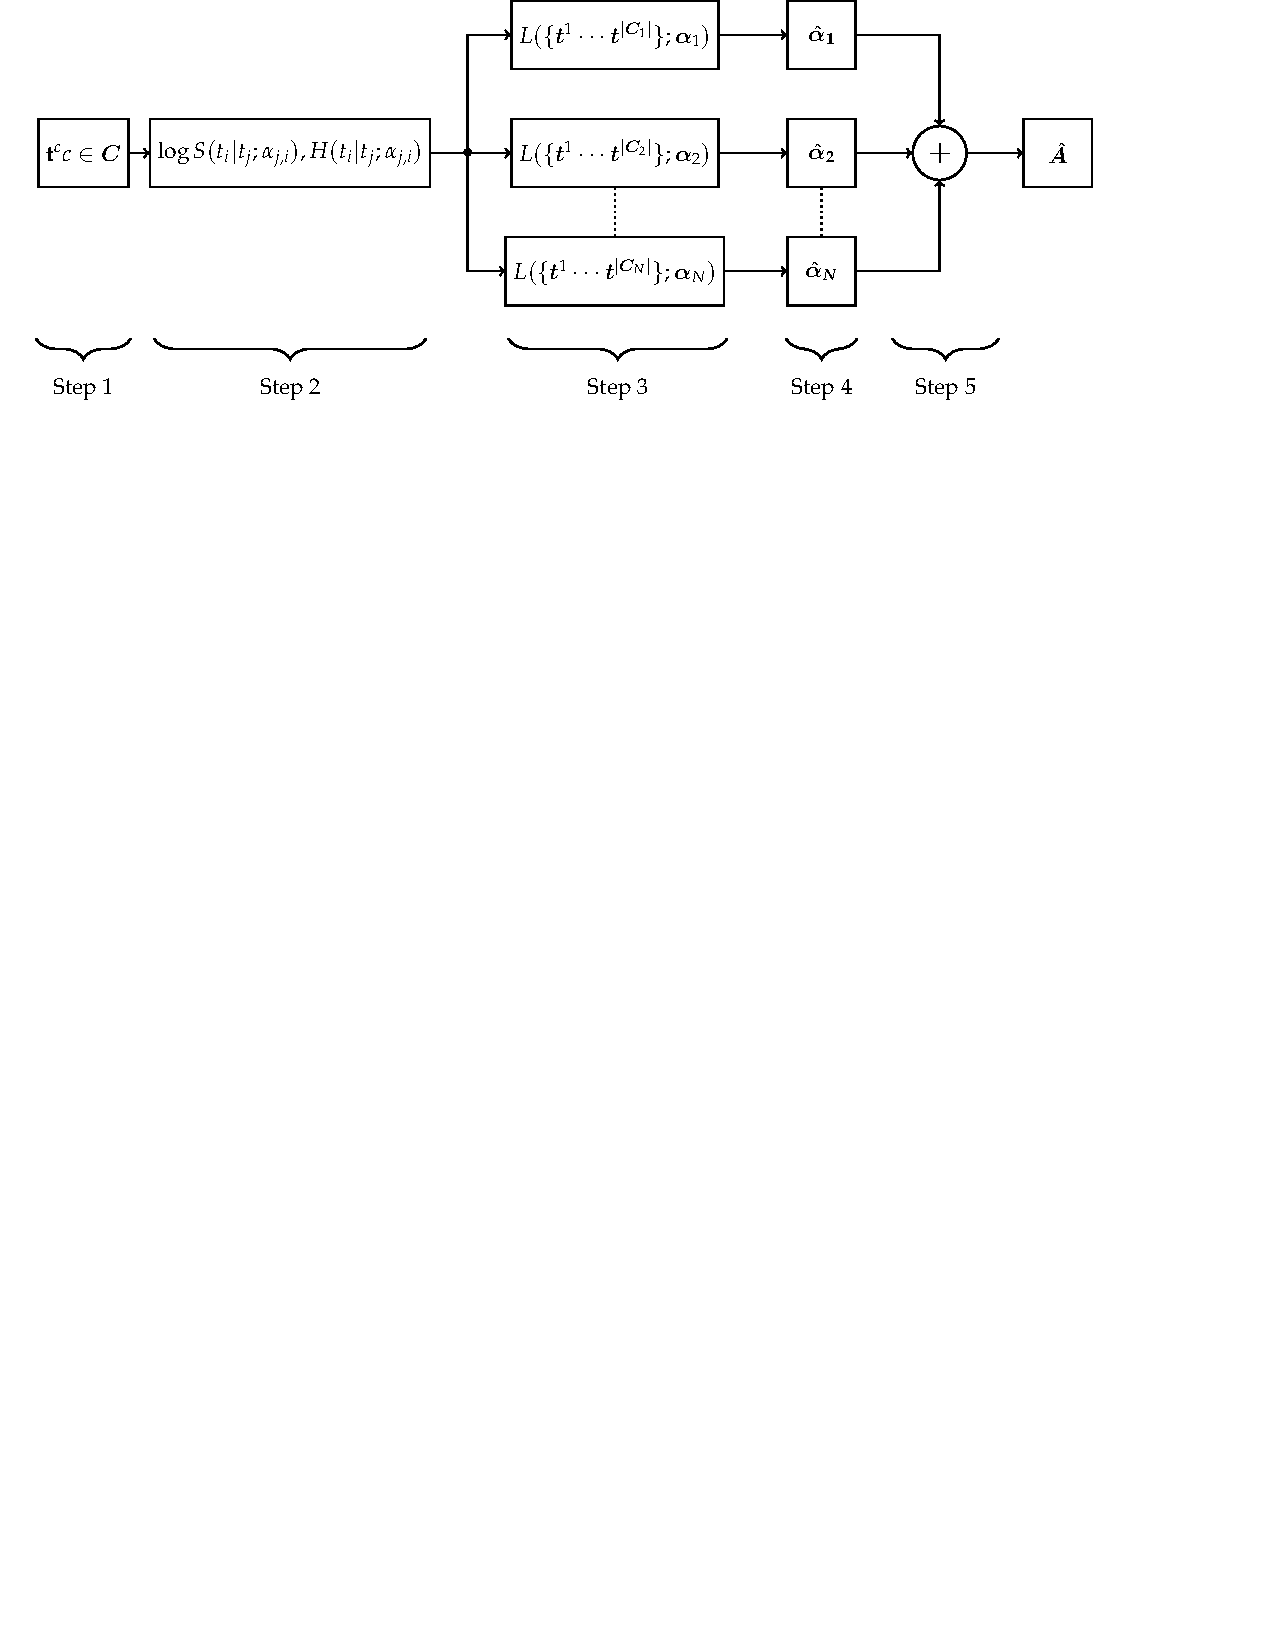
\includegraphics[trim={0 21cm 0 0}, width=\linewidth]{diagram_parallelization.pdf}
  \caption{Diagram of the NetRate parallelization process} 
	\label{fig:diagram_parallelization}
\end{figure}

Originally, the algorithm computed steps 3 and 4 sequentially. Once the transmission rates of a row of the adjacency matrix were computed, it continued with the following one. However, in a parallelized NetRate, they are all computed at the same time with step 5 also involving the stacking of each of the \(\bm{\hat{\alpha}}_{n}\) vectors to form the matrix \(\bm{\hat{A}}\).
The components in step 2 correspond to the ones seen in Eq.\ref{eq:solution_netrate} and whose solution is the assembled version of the one in step 3.\\

Once the structure of the algorithm is laid out, it still remains to plan how each of the jobs in steps 3 and 4 are will be assigned to the available processors. Not all the jobs take the same amount of time to be computed because they heavily depend on the number of cascades for their given node. As an illustration, a network of 10 neurons is simulated, and the number of cascades belonging to each node is shown in Eq.\ref{eq:num_cascades}. 

\begin{equation}
	\centering
	NoC = \{12, 21, 62, 166, 21, 67, 17, 30, 18, 81\}
	\label{eq:num_cascades}
\end{equation}

The mean of the distribution is 49 and the standard deviation 46. This means that the number of cascades differs significantly from node to node and that an appropriate way of distributing the jobs is required in order to keep all processors similarly busy. This is necessary because the whole algorithm will not finish until the last processor has estimated the weight parameters belonging to the last node. \\

Let \(M\) be the number of processors and \(N\) the number of nodes, where \(N > M\). The first \(M\) with the largest number of cascades are assigned in order to each of the processors. Each of the remaining \(N-M\) nodes is assigned to the processors following Eq.\ref{eq:argmin_processor}.

\begin{equation}
	\centering
	argmin_{n} \text{ } p_{i} + NoC_{n}, 
	\label{eq:argmin_processor}
\end{equation}

Where \(i \in [0,M]\) is the processor number, \(n \in [0, N - M]\) the node index and \(p_{i}\) is the sum of all the number of cascades assigned to processor \(i\). This method ensures that each of the processors has as close number of nodes as possible. Using Eq.\ref{eq:num_cascades} with \(N=10\), the distribution among \(M = 4\) processors becomes:

\begin{equation}
	\centering
	p_{1} = \{166\}, p_{2} = \{81, 21, 12\}, p_{3} = \{67, 21, 18\}, p_{4} = \{62, 30, 17\}
	\label{eq:distribution_processors}
\end{equation}

The resulting number of cascades for each of the processors becomes 166, 114, 106 and 109, respectively. This is a more balanced distribution than if the nodes had been assigned in any other way. \\

It remains to clarify in which order each of the nodes must be computed. One constraint that limits the algorithm is memory. The larger the number of cascades that need to be computed, the more memory is required for the algorithm to compute the weights. The relationship between the number of cascades and size of the network is exponential and, as it grows, NetRate makes use of a larger amount of memory. Each of the processors requires its own memory to perform NetRate in parallel. Thus, it becomes prohibitive to use several processors at the same time for large networks. However, some minor adjustments can be made to increase the capability of a parallelized NetRate by choosing which nodes are computed first. If all the largest nodes are computed at the same time the computer will not be able to finish the task for a sufficiently big network. For this reason, half of the processors will start with the nodes whose number of cascades is the lowest. The other half will do the opposite and compute the ones with the highest number of cascades. This way, the number of cascades computed at any given moment is levelled out and the likelihood of sudden spikes of memory usage are reduced. \\

As mentioned above, the CVX package cannot be parallelized naturally. Since the previous attempts to do so failed \cite{pranav_report}, a new method had to be implemented. For this project, instead of parallelizing NetRate from within MATLAB, several MATLAB instances are opened that work independently of each other. Each of these instances outputs a csv file and they are all combined by a Python script at the end of the computation. 

\subsection{Speed improvement results}

In this section the speed performance of the parallelized NetRate is evaluated. The computation time of NetRate for networks of different sizes, a stimulation period of 4000 ms and using 1, 4 and 8 processors is displayed in figure \ref{fig:speed_netrate}. Due to memory constraints of the computer, only up to 40 nodes were evaluated. As explained above, the more processors used at the time the more memory is required and this made the algorithm stall when using 8 processors in a network of 50 neurons.\\

\begin{figure}
\centering
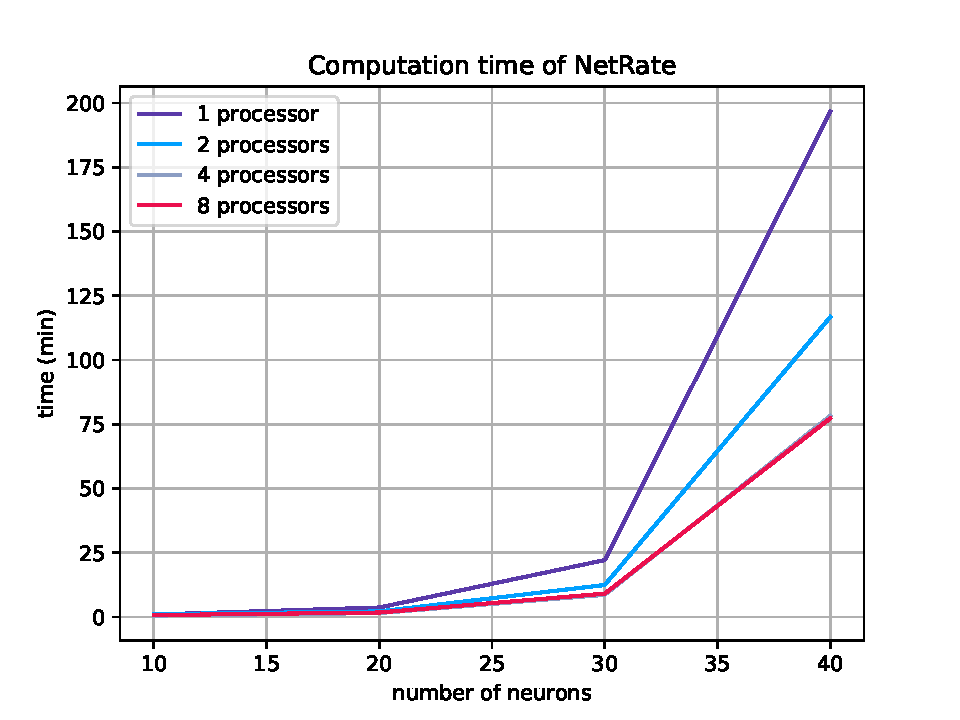
\includegraphics[width=0.8\linewidth]{computation_time_netrate.pdf}
\caption{Computation time of NetRate}
\label{fig:speed_netrate}
\end{figure}

There is a significant improvement in the speed of the algorithm when comparing 1 processor to 4 and 8 processors. For 30 neurons, it takes 22, 8 and 9 minutes for 1, 4 and 8 processors whereas for 40 neurons, it takes 196, 77 and 78 minutes. Although these are good results, they are far from ideal. 
Firstly, the time it takes to do the computation with 4 processors is not 4 times faster than with just one processor. It is, in fact, approximately 2.6 for the networks with 30 and 40 neurons. 
Moreover, using 8 processors instead of 4 results in no speed improvement for any of the networks. It is difficult to understand this behaviour because deeper analysis shows that all 8 processors are busy during the computation of the algorithm. One possible explanation is that the only steps that are actually being parallelized are number 3 from figure \ref{fig:diagram_parallelization}, where the optimization problem in \ref{eq:optimization_netrate} for each of the rows of the adjacency matrix is built, and half of step 4, where the CVX package is used but the solver has not been called. This means that the solver in the CVX package is a shared resource among all the running MATLAB instances and that each of the processors waits in a queue to compute its own row of the adjacency matrix. Further investigation into this hypothesis leads in this direction: when printing the progress of the optimization solver SDPT3, there is a linear behaviour i.e all processes print in an orderly fashion and there is no overlapping between them. However, further research into this issue must be carried out.\\

In this section it has been described what the steps of NetRate are, how the parallelization is implemented and what its limitations are. It is necessary to have a fast algorithm for it to be used with large networks. Finally, it was shown that although there is a significant improvement in the speed of NetRate, it is not as good as desired, and it also poses further restrictions on memory usage.  
